% Universidade Federal de Campina Grande
% Modelo de Proposta de Disserta��o de Mestrado em Ciencia da Computacao
%
% Feito por: Ana Cristina Alves de Oliveira
% (cristina@dsc.ufcg.edu.br - orientador: Francisco Brasileiro)
% Fevereiro de 2006

% E necessario o arquivo "algorithm.sty", se for construir algoritmos

% Adaptado por: Leandro Dias da Silva
% (leandrodias@ic.ufal.br - Coordenador do PPGI)
% Junho de 2013

% readaptado por: Ailton Felix, Lucas Lins, Marcelo Oliveira
% (oliveiramc@ic.ufal.br - Coordenador do PPGI)
% em Julho de 2018

% \documentclass[titlepage,12pt]{article}

\documentclass[titlepage,12pt,openright,oneside,sumario=tradicional,a4paper,english,article]{abntex2}

\chapterstyle{default}
%\usepackage[a4paper, left=3cm,top=3cm,right=2cm,bottom=2cm]{geometry}

\usepackage{color}
\usepackage{longtable}
\usepackage{lipsum} 
\usepackage{tabulary}
\usepackage{tabu}
\usepackage{ltablex}

%\usepackage[portuges,english]{babel}

%Portuguese-specific commands
%--------------------------------------
%\usepackage[english,brazil,portuguese]{babel}
%--------------------------------------
 
%Acentuação em UTF8
\usepackage[utf8]{inputenc}            % 
%\usepackage[latin1]{inputenc}

\usepackage{times}
%\usepackage[latin1]{inputenc}
\usepackage[T1]{fontenc}
\usepackage{fancyheadings}
\usepackage{fancyvrb}

\usepackage{algorithmic}
\usepackage[nothing]{algorithm}
\usepackage{latexsym}
\usepackage{indentfirst}                 % indenta os primeiros parágrafos
\usepackage{amsmath}  %texto no modo math
%\usepackage[colorlinks,pdftex,pdfpagelabels=false]{hyperref} % Inclusão de links  

\usepackage{graphicx,url}
\usepackage{import}
\usepackage{booktabs}

\usepackage{lscape}
\usepackage{flushend}
\usepackage{longtable}
\usepackage[table,xcdraw]{xcolor}
\usepackage{multirow}
\usepackage{color, colortbl}
\usepackage{todonotes}

\usepackage{pdfpages}

\hypersetup{
		colorlinks=false}%,     		% false: boxed links; true: colored links
		%linkcolor=blue,        		% color of internal links
		%citecolor=blue,        		% color of links to bibliography
		%filecolor=magenta,     		% color of file links
		%urlcolor=blue}

\usepackage{hyperref} % controla a formação do índice

%Referencias na forma da ABNT
\usepackage[alf]{abntex2cite} 

\sloppy

% Comandos de estilo e espacamento ----------------------------------------
\newlength{\defbaselineskip}
\setlength{\defbaselineskip}{\baselineskip}
\newcommand{\setlinespacing}[1]%
           {\setlength{\baselineskip}{#1 \defbaselineskip}}

\setcounter{topnumber}{2}
\renewcommand{\topfraction}{.7}
\setcounter{bottomnumber}{1}
\renewcommand{\bottomfraction}{.3}
\setcounter{totalnumber}{3}
\renewcommand{\textfraction}{.2}
\renewcommand{\floatpagefraction}{.5}
\setcounter{dbltopnumber}{2}
\renewcommand{\dbltopfraction}{.7}
\renewcommand{\dblfloatpagefraction}{.5}
%
\oddsidemargin -28pt
\evensidemargin -28pt
\marginparwidth 50pt
\marginparsep 5pt
\topmargin -27pt
\hoffset 15mm
\textheight 237mm
\textwidth 155mm
\renewcommand{\baselinestretch}{1.5}
%

\newenvironment{braced}
 {\par\smallskip\hbox to\columnwidth\bgroup
  \hss$\left\{\begin{minipage}{\columnwidth}}
 {\end{minipage}\right\}$\hss\egroup\smallskip}


% Color definitions (RGB model)
\definecolor{mycolor1}{rgb}{0.753,0.753,0.753}

\begin{document}

% Primeira Folha do Documento %%%%%%%%%%%%%%%%%%%%%%%%%%%%%%%%%%%%%%%%%%%%%


%
% Cover
%
\selectlanguage{english}

\import{sections/}{capa.tex}

\newpage
\thispagestyle{empty}

%
% Folha de Rosto
%

\import{sections/}{folha-de-rosto.tex}
\thispagestyle{empty}

%
% Filha catalográfica
%

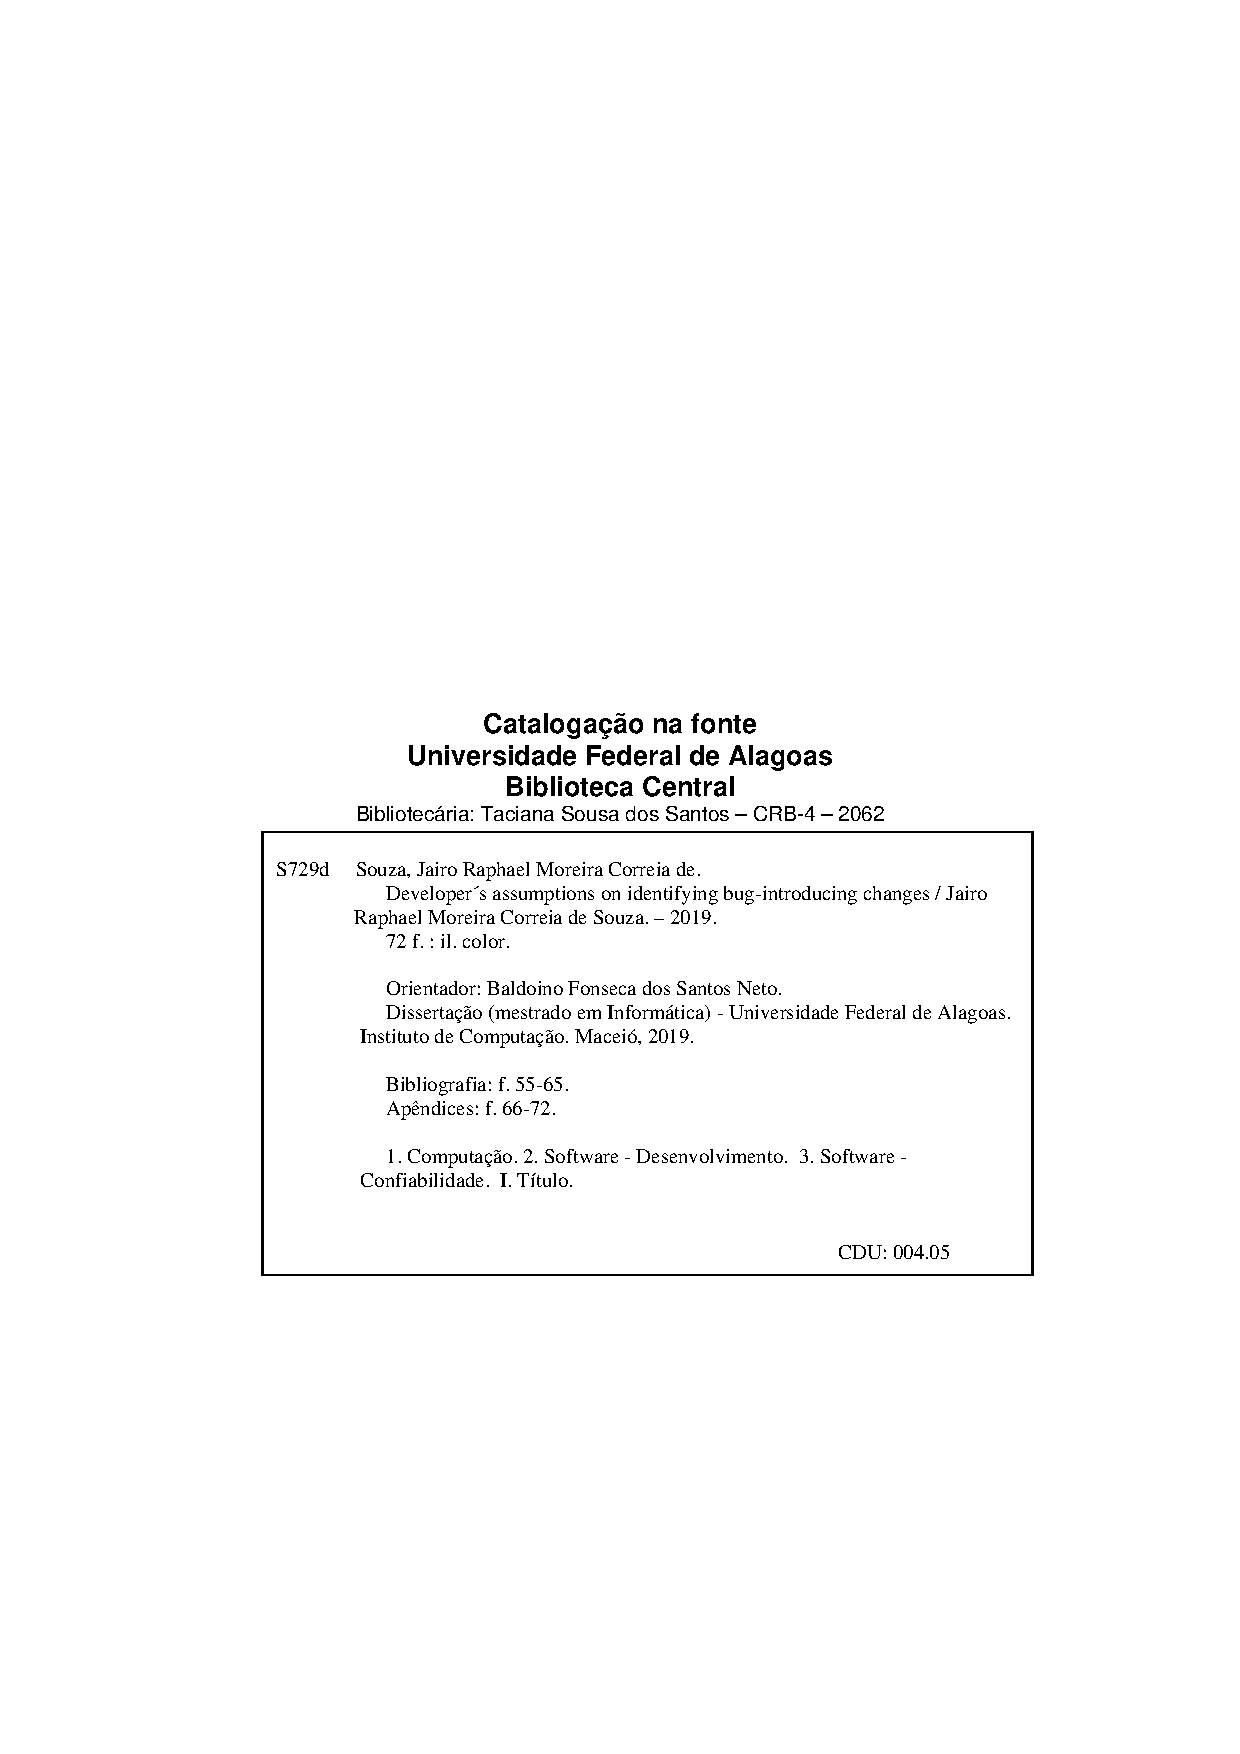
\includepdf[pages=-,pagecommand={}]{Fichacat7910-2019.pdf}
%\import{sections/}{folha-aprovacao.tex}
\newpage
\thispagestyle{empty}

%
% Folha de aprovação para ser impressa e preenchida pela banca examinadora
%

%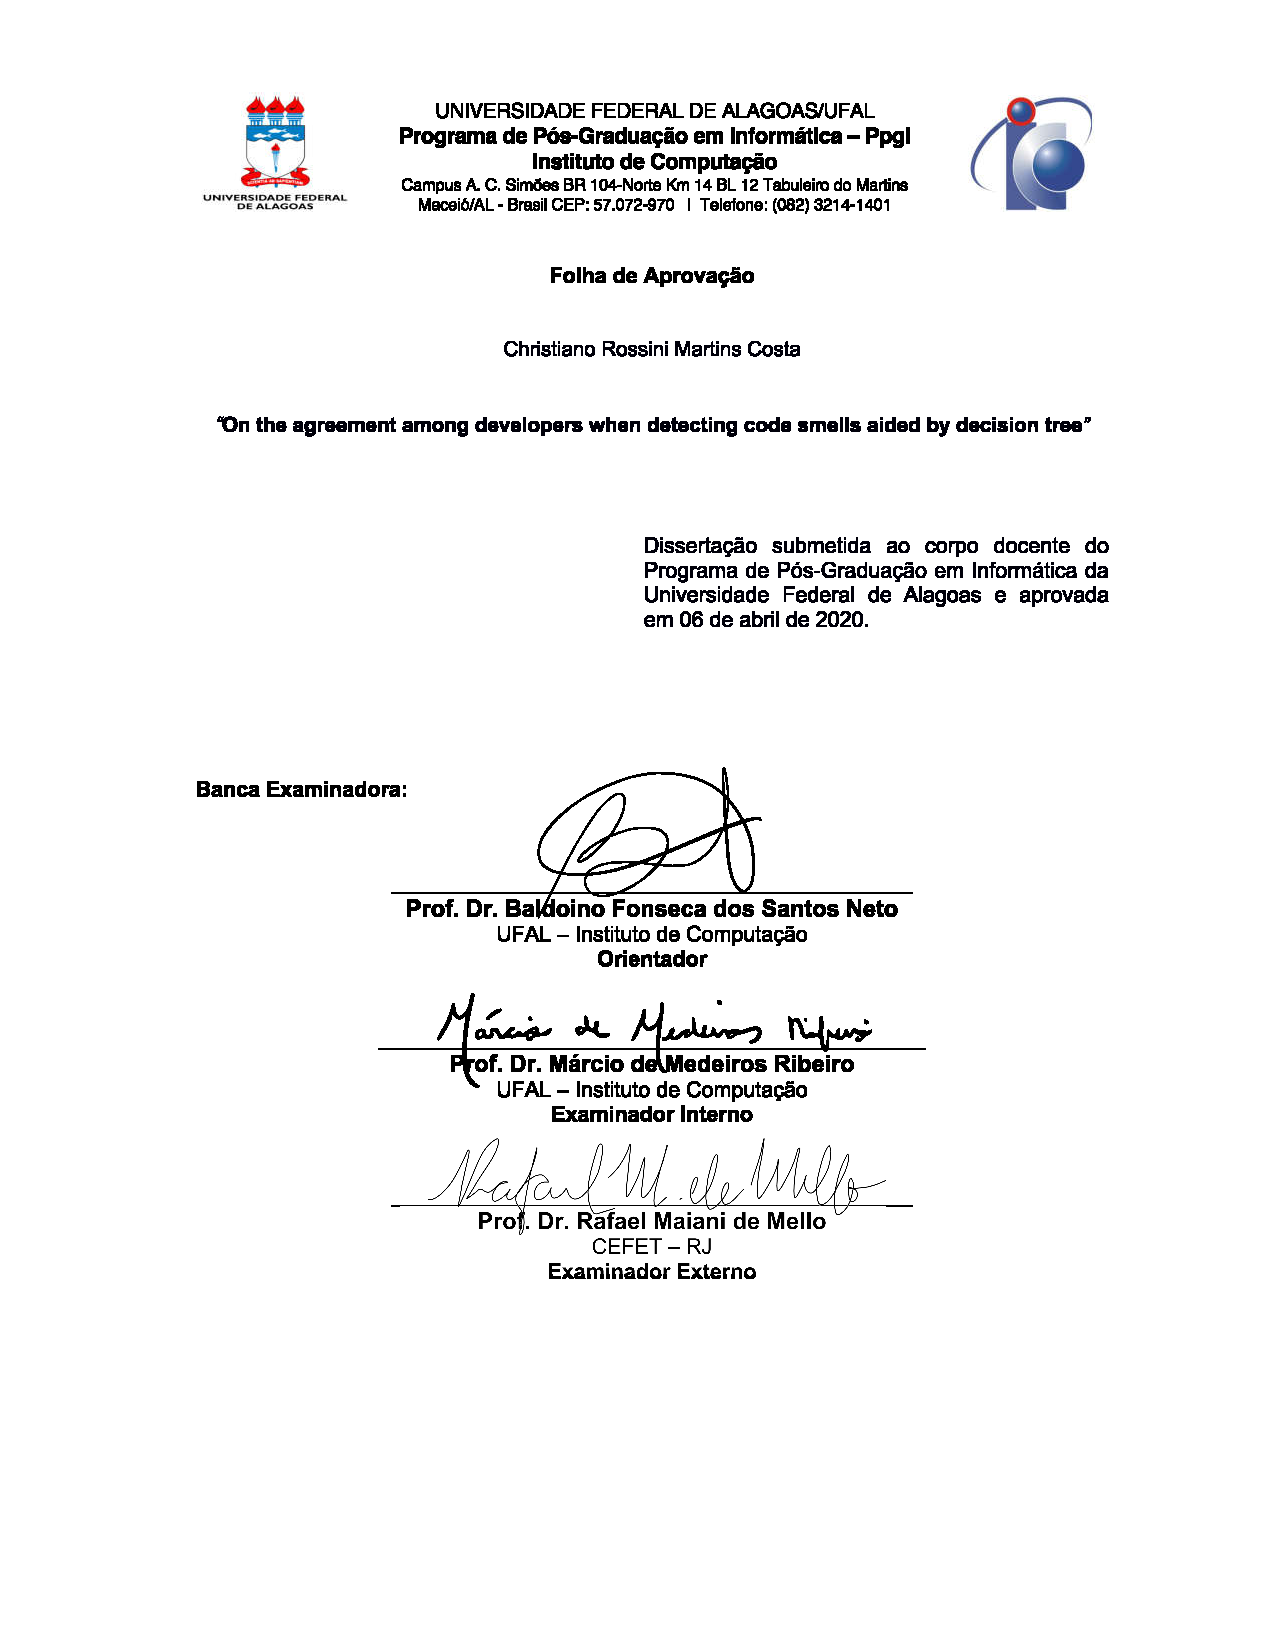
\includepdf[pages=-,pagecommand={}]{folha_aprovacao.pdf}
\import{sections/}{folha-aprovacao.tex}
\newpage
\thispagestyle{empty}

%
% Dedicatória
%

\import{sections/}{dedicatoria.tex}

%%%%%%%%%%%%%%%%%%%%%%%%%%%%%%%%%%%%%%%%%%%%%%%%%%%%%%%%%%%%%%%%%%%%%%%%%%%%%%%

\newpage
\cleardoublepage

%%%%%%%%%%%%%%%%%%%%%%%%%%%%%%%%%%%%%%%%%%%%%%%%%%%%%%%%%%%%%%%%%%%%%%%%%%%%%%%%

% ConFigura os n�meros das p�ginas para algarismos romanos
\pagestyle{plain}
\pagenumbering{roman}

\newpage
\thispagestyle{empty}

\import{sections/}{agradecimentos.tex}
\thispagestyle{plain}
\newpage

%Resumo:
\import{sections/}{resumo.tex}
\thispagestyle{plain}

%Abstract:
\newpage
\import{sections/}{abstract.tex}
\newpage

\listoffigures
\newpage

\listoftables
\newpage

\tableofcontents
\newpage
% Inclui a lista de algoritmos
%\incluilistadealgoritmos


% Corpo do documento -------------------

% ConFigura os n�meros das p�ginas para algarismos indo-arabicos
\pagestyle{plain}
\setcounter{page}{1}
\pagenumbering{arabic}

%%%%%%%%%%%%%%%%%%%%%%%%%%%%%%%%%%%%%%%%%%%%%%%%%%%%%%%%%%%%%%%%%%%%%%%%%%%%%%%%
% Definicao do cabecalho: secao do lado esquerdo e numero da pagina do lado direito
\pagestyle{fancy}
\addtolength{\headwidth}{\marginparsep}\addtolength{\headwidth}{\marginparwidth}\headwidth=\textwidth
\renewcommand{\sectionmark}[1]{\markboth{#1}{}}
\renewcommand{\sectionmark}[1]{\markright{\thesection\ #1}}\lhead[\fancyplain{}{\bfseries\thepage}]%
         {\fancyplain{}{\emph{\rightmark}}}\rhead[\fancyplain{}{\bfseries\leftmark}]%
             {\fancyplain{}{\bfseries\thepage}}\cfoot{}

%%%%%%%%%%%%%%%%%%%%%%%%%%%%%%%%%%%%%%%%%%%%%%%%%%%%%%%%%%%%%%%%%%%%%%%%%%%%%%%%
\import{sections/}{01-introduction.tex}
\newpage
\import{sections/}{02-background.tex}
\newpage
\import{sections/}{03-study-design.tex}
\newpage
\import{sections/}{04-results.tex}
\newpage
\import{sections/}{05-discussions.tex}
\newpage
\import{sections/}{06-related-work.tex}
\newpage
\import{sections/}{07-threats.tex}
\newpage
\import{sections/}{08-conclusion.tex}
\newpage

%%%%%%%%%%%%%%%%%%%%%%%%%%%%%%%%%%%%%%%%%%%%%%%%%%%%%%%%%%%%%%%%%%%%%%%%%%%%%%%%
%% BIbliografia

% \bibliographystyle{abntex2}
%\bibliographystyle{abbrv} % estilo de bibliografia
\bibliography{mybibfile} % arquivos com as entradas bib.

\newpage
%%%%%%%%%%%%%%%%%%%%%%%%%%%%%%%%%%%%%%%%%%%%%%%%%%%%%%%%%%%%%%%%%%%%%%%%%%%%%%%%
%\pagestyle{plain}
\import{sections/}{09-appendix.tex}

% \section{Título do apêndice B}
% \label{ape:apeB}

% Incluir o texto do apêndice aqui, caso haja.


\end{document}
